% !TeX root=../main.tex
\chapter{روش پیشنهادی}
%\thispagestyle{empty} 
\section{مقدمه} 

در این بخش قسمت های مختلف الگوریتم پیشنهادی برای تشخیص نوع فعالیت انسان در تک تصویر بررسی می‌شود. برای درک نوع فعالیت درحال انجام، عوامل مختلفی می‌توانند دخیل ‌باشند. ازجمله طرز ایستادن شخص که ژست انسان را نشان می‌دهد،‌ صحنه‌ای که فعالیت درآن درحال انجام است مثل زمین تینس در بازی تنیس و یا اشیاء که انسان با آن تعامل دارد مثل "لیوان" در فعالیت "نوشیدن آب".\\
روش پیشنهادی از چندین مرحله تشکیل می‌شود که درادامه به تفصیل بررسی می‌شود. ترکیب ژست با موقعیت بدنی داخل یک مکانیزم توجه از جمله مهم ترین مراحل بشمار می‌رود و چالش‌های زیادی مانند تخمین ژست در حالت های مختلف انسان،‌ به‌دست آوردن ناحیه های کلیدی،‌ %
\gls{Occlusion}
بعضی اجزاء بدن و عوامل گمراه کننده برای شبکه وجود دارد.\\
روش ها و الگوریتم‌های مختلفی برای تشخص فعالیت در تک تصویر وجود دارد. روش‌های مبتنی بر موقعیت بدنی و ژست، موقعیت بدنی و اشیاء، اشیاء و ژست و روش ترکیبی موقعیت بدنی، ژست و اشیاء که جزء بهترین روش‌‌ها بشمار می‌رود و اغلب به نتایج امیداورکننده رسیده است. هرکدام از این روش‌‌ها و الگوریتم‌ها دارای مزایا و معایبی هستند که هرکاربرد خاصی باید الگوریتم تشخیص حرکت مناسبی را درنظر گرفت.\\
با درنظر گرفتن چالش‌های موجود در کاربرد مورد نظر و نقاط ضعف و قوت روش‌های موجود از موقعیت بدنی،‌ اشیاء و ژست برای تشخیص فعالیت در تک تصویر استفاده شده است. برای ترکیب ویژگی‌های ظاهری انسان که موقعیت بدنی را نشان می‌دهد با ژست از مکانیزم توجه استفاده شده است. همچنین دراین فصل درباره نحوه محاسبه یک بردار ویژگی برای ژست انسان در یک روش بدون مکانیزم توجه برای مقایسه با مکانیزم توجه بحث شده است.

\section{مراحل الگوریتم پیشنهادی}

\begin{figure}[ht]
	\centerline{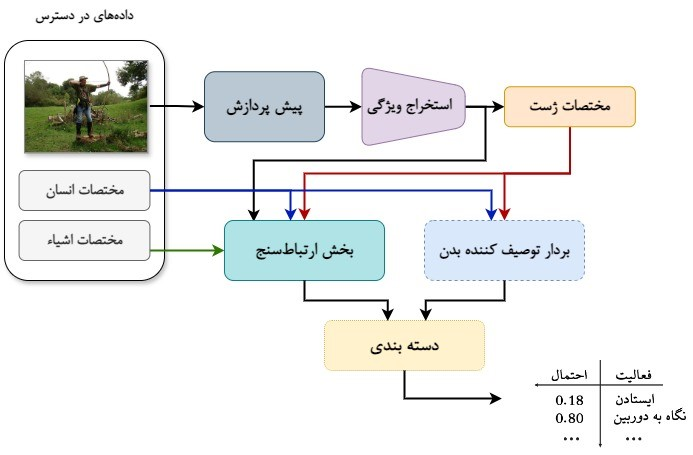
\includegraphics[width=0.8\textwidth]{Flowchart_whole}}
	\caption{ساختار کلی شبکه پیشنهادی
	}
	\label{fig:Flowchart_whole}
\end{figure}
شکل %
\ref{fig:Flowchart_whole}
ساختار کلی طراحی شده را نشان می‌دهد. از یک بخش ارتباط‌سنج %
\gls{RelationModule}
برای ترکیب ویژگی‌های انسان با اشیاء که شبکه ResNet کار استخراج ویژگی را انجام می‌دهد،‌ استفاده شده است. 
پس از انجام پیش‌ پردازش‌های لازم جهت بهبود کیفیت تصویر، غلبه بر مشکلات انسداد، نرمال سازی و تقویت داده‌ها، نواحی مهم از جمله ناحیه انسان، اشیاء و اجزاء بدن از تصویر بریده می‌شود و ویژگی های آنها از یک شبکه عصبی عمیق استخراج می‌شود. همچنین برخی تغییرات در رنگ و اندازه تصویر داده می‌شود تا داده‌ها تنوع بیشتری به خود بگیرند که این تغییر رنگ و اندازه یک سری چالش‌هایی نیز دارد که در بخش %
\ref{pishe_pishnehadi}
بیشتر توضیح داده می‌شود.
از ویژگی‌های استخراج شده جهت تخمین مختصات ژست استفاده می‌شود و سپس این مختصات در کنار مختصات انسان و اشیاء در بخش‌های بعدی استفاده می‌شود. همانطور که در شکل %
\ref{fig:Flowchart_whole}
نشان داده شده، بخش ارتباط‌سنج از سه مختصات موقعیت بدنی انسان، اشیاء و ژست استفاده می‌کند که یک خروجی معنادار و ارتباط‌ یافته تولید کند. مسیر بردار توصیف کننده بدن، یک روش پیشنهادی دراین پایان نامه است که از مختصات ژست و موقعیت بدنی استفاده می‌کند که یک بردار از ژست تشکیل دهد. در ادامه خروجی این دو بخش باهم ترکیب شده و یک دسته‌بندی انجام می‌شود.
البته درون بخش ارتباط‌سنج یک نوعی ژست با موقعیت بدنی ‌انجام می‌شود که به عنوان بخش اضافی بررسی می‌شود.

\subsection{مرحله پیش پردازش}\label{pishe_pishnehadi}

در این مرحله باید ابتدا کانال تصویر رنگی از هرکانالی که است به RGB تغییر پیدا کند. اصولاً شبکه‌های عصبی با این ساختار بهتر به نتیجه می‌رسند. تصاویر موجود اغلب کیفیت مناسبی دارند بااین حال برخی از تصاویر وضوح بسیار پایینی دارند که شناسایی شخص دراین تصویر حتی برای انسان نیز کار دشواری است. این تصاویر از فهرست داده ها حذف شده است.
در ادامه مراحل پیش پردازش در چند بخش مورد بررسی قرار گرفته است:
\subsubsection{نرمال سازی داده}

یکی از ابعاد اساسی در پیش‌پردازش تصاویر، نرمال‌سازی است که بهبود قابلیت‌ها و عملکرد مدل‌ها را تضمین می‌کند. تصاویری که به صورت ورودی به مدل‌های یادگیری عمیق و الگوریتم‌های تصویری داده می‌شوند، معمولاً شامل متغیرهایی مانند روشنایی، کنتراست، و زاویه‌های مختلف هستند. این تغییرات متنوع و گاهی پیچیده در تصاویر می‌توانند باعث مشکلات در یادگیری مدل‌ها شوند. بنابراین، نیاز به یک مرحله پیش‌پردازش قوی و موثر که تصاویر را به یک وضعیت استاندارد و قابل تشخیص تبدیل کند، اساسی است.

نرمال‌سازی تصاویر یکی از اصول اساسی در پیش‌پردازش است که بهبودی در تطبیق مدل با داده‌ها و افزایش قابلیت تعمیم مدل به داده‌های جدید را ایجاد می‌کند. این مرحله اقدام به تعیین وضعیت استاندارد برای تصاویر دارد تا مدل بتواند با ورودی‌های متفاوت و شرایط مختلف بهتر سازگار شود.

شکل %
\ref{fig:normalization_no_norm}
یک نمونه از روند یادگیری شبکه عصبی با ساختار داده‌های نرمال‌ شده و نرمال نشده را نشان می‌دهد. داده‌های نرمال نشده حرکت‌های زیگزاگی را در طی آموزش دارند و برای رسیدن به جواب بهینه تعداد گام‌های بیشتری را طی می‌کنند درحالی که داده‌های نرمال شده شکل حرکتی منظم‌تری دارند. طول این محور با پارامتر %
\gls{LearningRate}
مشخص می‌شود. بنابراین در داده‌های نرمال نشده نرخ یادگیری بزرگتری نیاز است تا مدل مسیر اولیه خود را پیدا کند و در گام‌های بعدی نرخ یادگیری ها متفاوت می‌شود درحالی که در داده نرمال شده،‌ باید یک نرخ یادگیری ثابت به جواب بهینه دست پیدا می‌کند.

\begin{figure}[ht]
	\centerline{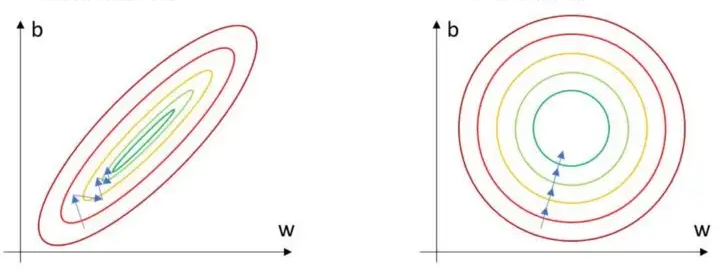
\includegraphics[width=0.8\textwidth]{normalization_no_norm}}
	\caption{فرآیند یادگیری شبکه عصبی با داده نرمال شده (راست) و داده نرمال نشده (چپ)
	 \cite{Normal_not_Normal}
	}
	\label{fig:normalization_no_norm}
\end{figure}

در ادامه توضیحات، به بررسی روش‌های مختلف نرمال‌سازی تصاویر پرداخته و سپس به بررسی یکی از روش‌های مفید‌ترین نرمال‌سازی، یعنی  نرمال‌سازی میانگین و واریانس، پرداخته خواهد شد. استفاده از  نرمال‌سازی میانگین و واریانس به عنوان یک روش مؤثر در نرمال‌سازی تصاویر در شبکه‌های عصبی اهمیت بیشتری یافته است و به بهبود سرعت و عملکرد آموزش مدل‌ها کمک زیادی می‌کند. همچنین درداخل شبکه از %
\gls{BatchNormalization}
 نیز جهت نرمال‌سازی استفاده شده است که ادامه بررسی می‌شود.
\begin{itemize}
	\item \textbf{نرمال سازی به روش :Min-Max }
	در این روش، مقادیر پیکسل‌ها به گونه‌ای تغییر می‌کنند که حداقل مقدار به صفر و حداکثر مقدار به یک تبدیل شوند. این نرمال‌سازی معمولاً برای تصاویری با دینامیک مقادیر محدود مفید است.
	\item \textbf{نرمال سازی به روش :Z-Score }
	 این روش تصویر را به نحوی نرمال‌سازی می‌کند که میانگین آن صفر و انحراف معیاری به یک تغییر یابد. این نرمال‌سازی اغلب برای تصاویری با توزیع‌های پیچیده استفاده می‌شود.
\end{itemize}
دو روش که در بالا گفته شد، یک سری معایبی دارند از جمله روی داده ها با توزیع گسترده و انحراف معیار‌های بزرگ عملکرد ضعیفی دارند همچنین در تصاویر با توزیع های غیر معمول چندان کارایی مطلوبی ندارند. دو روش نرمال‌سازی استفاده شده در زیر توضیح داده می‌شود.

$\bullet$ \textbf{نرمال‌سازی میانگین و واریانس}
\LTRfootnote{Mean and  Variance Normalization}
:\\
در این روش، میانگین تمام پیکسل‌ها از تصویر کم می‌شود تا میانگین آن به صفر برسد. سپس واریانس نیز تا یک مقداری تغییر می‌کند. این کار به مدل کمک می‌کند تا با داده‌هایی که به صورت معیارهای نرمال سازی شده هماهنگ شود.

طبق فرمول 
 \ref{eq:normalizaion}
داده‌های نرمال‌ شده از تفریق میانگین %
$\mu$
 از داده‌ها و تقسیم شدن بر انحراف معیار %
 $\sigma$ 
 به دست می‌آید.
\begin{equation}
	\label{eq:normalizaion}
	x:=\frac{x-\mu}{\sigma}
\end{equation}

انحراف معیار در اینجا از فرمول %
\ref{eq:enheraf_meyar}
 بدست می‌آید که %
 $E[X]$
  میانگین را نشان می‌دهد.
  \begin{equation}
  	\label{eq:enheraf_meyar}
  	  \sigma=\sqrt{E\left[X^2\right]-(E[X])^2}
  \end{equation}
  
$\bullet$ \textbf{نرمال‌سازی دسته‌ای در ساختار شبکه عصبی}
:\\
در شبکه‌های عصبی، از نرمال سازی دسته‌ای به عنوان یک لایه نرمال‌سازی استفاده می‌شود. این لایه برای هر دسته از داده‌ها، میانگین و انحراف معیار محاسبه کرده و مقادیر ورودی را مطابق با آنها نرمال‌سازی می‌کند. 
استفاده از نرمال‌سازی دسته‌ای به عنوان یک روش مفید در نرمال‌سازی تصاویر به ویژه در شبکه‌های عصبی توصیه می‌شود. این روش نه تنها باعث نرمال‌سازی میانگین و انحراف معیار است، بلکه به شبکه عصبی کمک می‌کند تا سریع‌تر و بهتر آموزش ببیند. نرمال‌سازی دسته‌ای همچنین مشکل %
\gls{VanishingGradients}
 را کاهش می‌دهد و از مشکل برخورد با مشکل %
\gls{ExplodingGradients}
 جلوگیری می‌کند. این روش بهبود قابل توجهی در سرعت و کارایی یادگیری شبکه‌های عصبی دارد و بنابراین در بسیاری از حوزه‌های بینایی ماشین مورد استفاده قرار می‌گیرد.
 
  \subsubsection{افزایش داده}
 در حوزه یادگیری عمیق و تشخیص فعالیت‌ها در تصاویر، پیش‌پردازش تصاویر با %
 \gls{DataAugmentation}
 یکی از مراحل حیاتی است که تاثیر قابل توجهی بر عملکرد مدل‌های یادگیری عمیق دارد. با توجه به محدودیت داده در بسیاری از موارد، افزایش داده به عنوان یک روش مؤثر و اساسی در بهبود دقت و قابلیت تعمیم مدل‌ها به مسائل واقعی و متنوع مورد استفاده قرار می‌گیرد.
 
 توسعه تکنولوژی و افزایش استفاده از شبکه‌های عصبی عمیق، نیاز به داده‌های بزرگ‌تر و متنوع‌تر را ایجاب کرده است. هرچند ممکن است در بعضی از حوزه‌ها داده‌های زیادی در دسترس باشد، اما در حوزه تشخیص فعالیت‌ها، اغلب با محدودیت داده مواجه هستیم. این مسئله می‌تواند منجر به بروز مشکلاتی مانند بیش‌برازش یا کم‌دادگانی شود که در نهایت باعث کاهش دقت و قابلیت تعمیم مدل می‌شود.

 \textbf{اهمیت افزایش داده:}

 با توجه به محدودیت داده در بسیاری از حوزه‌ها، افزایش داده به عنوان رویکردی مؤثر در جلوگیری از بروز مشکلاتی مانند %
\gls{Overfitting}
  یا کم‌دادگانی به شمار می‌آید. این روش از طریق تولید نمونه‌های جدید از داده‌های موجود، مدل را به موارد مختلف و ناشناخته مواجه می‌کند و این امکان را فراهم می‌کند که مدل در شرایط مختلف عملکرد مناسبی از خود نشان دهد. افزایش داده به ویژه در مواردی که داده محدود است، کمک می‌کند تا مدل به طور کلی عملکرد بهتری داشته باشد. 
  
  در ادامه، به بررسی یک‌سری ملاحظات درنظرگرفته شده در فرآیند افزایش داده و نیز ارائه راهکارهایی برای اجرای بهینه این عملیات می‌پردازیم.
  
\begin{itemize}
	\item \textbf{تطبیق با خصوصیات مسئله:}
	تکنیک‌های افزایش داده باید خصوصیات مسئله و نوع داده را درنظر بگیرند. مثلاً در تشخیص فعالیت‌ها، چرخش تصویر ممکن است برای تصاویر فعالیت انسانی مناسب‌تر باشد.
	
	\item \textbf{پیش‌پردازش همراه با افزایش داده:}
	برخی از تکنیک‌های پیش‌پردازش مانند نرمال‌سازی تصویر می‌توانند با افزایش داده ترکیب شوند و به بهبود تعمیم مدل کمک کنند.
	
	\item \textbf{ارزیابی اثربخشی تغییرات:}
	ارزیابی دقیق تأثیر هر تغییر در دقت و عملکرد مدل ضروری است تا تصمیمات بهینه‌تر در انتخاب تکنیک‌ها گرفته شود.
	
	\item \textbf{استفاده از چند تکنیک به صورت ترکیبی:}
	استفاده از ترکیب چند تکنیک افزایش داده می‌تواند به تنوع بیشتر و بهبود قابلیت تعمیم مدل منجر شود.
\end{itemize}

در روش پیشنهادی از 4 نوع افزایش داده یا تغییرات داده استفاده شده است که درزیر به آنها اشاره می‌شود:

\textbf{1. \gls{Rotation}}
\textbf{:}
تصویر با زاویه‌های تصادفی چرخش داده می‌شود. این کار به مدل کمک می‌کند تا اجسام از هر زاویه‌ای تشخیص داده شوند.

\textbf{2. \gls{Scaling}}
\textbf{:}
تصویر به اندازه‌های تصادفی کوچکتر یا بزرگتر شده و سپس به اندازه مورد نظر برگردانده می‌شود. این تغییرات موجب بهبود تعمیم‌پذیری مدل می‌شود.

\textbf{3.  \gls{HVFlip}}
\textbf{:}
تصویر به صورت افقی یا عمودی بازانعکاس داده می‌شود. این تغییرات باعث افزایش تنوع داده و تشخیص صحیح‌تر اجسام می‌شود.

\textbf{4.  \gls{ColorJittering}}
\textbf{:}
اعمال تغییرات تصادفی در رنگ‌های تصویر مانند تغییر روشنایی، کنتراست و اشباع. این کار به مدل کمک می‌کند تا با تنوع بیشتری در برابر تغییرات نوری مقاوم باشد.

انجام برخی از این تغییرات روی تصویر ممکن است منجبر به یک سری خطاهای دیگر شود. تغییراتی مانند چرخش و تغییر اندازه باعث می‌شود %
\glspl{BoundingBox}
که برای اشیاء و انسان دردسترس است با خطا مواجه شود. برای غلبه براین مشکل باید تغییراتی که باعث می‌شود اندازه تصویر تغییرات کند روی %
\glspl{BoundingBox}
 موجود نیز اعمال شود. 

دو نمونه از تصاویر بدون اعمال تغییرات و با اعمال تغییرات به ترتیب در شکل %
 \ref{fig:no_album}
 و
\ref{fig:with_album}
نشان داده شده است. 
\begin{figure}
	\centering
	\subfloat[بدون اعمال تغییرات
	]{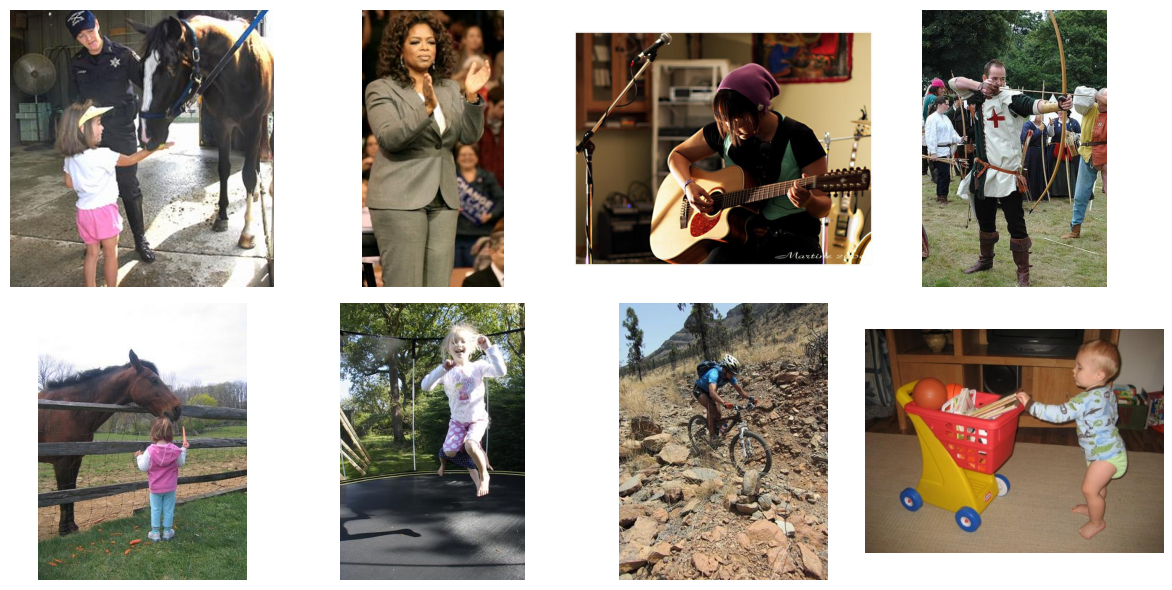
\includegraphics[width=0.75\textwidth]{no_album}
	\label{fig:no_album}}
	\hfill
	\subfloat[با اعمال تغییرات
	]{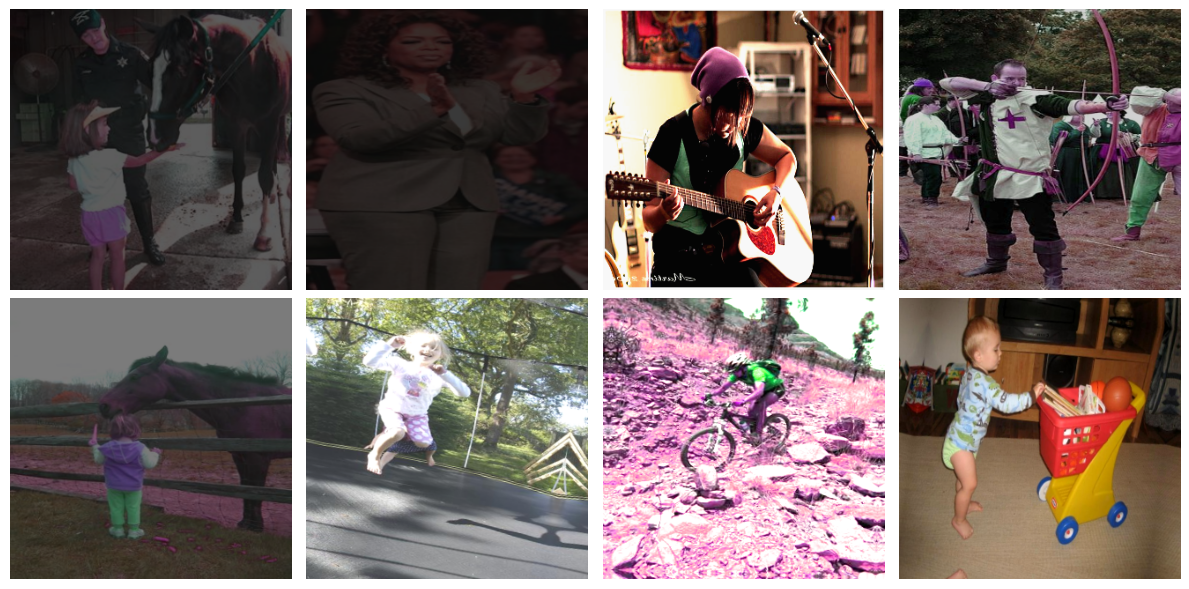
\includegraphics[width=0.75\textwidth]{with_album}
	\label{fig:with_album}}
	\hfill
	\caption{یک سری تصاویر با اعمال تغییرات و بدون اعمال تغییرات}
	\label{fig:with_no_album}
\end{figure}
همانطور که مشخص است اندازه تمامی تصاویر به یک اندازه مشخص درآمده است و هدف از اینکه اندازه تمامی تصاویر یکسان است این است که شبکه نمی‌تواند اندازه‌های مختلف را اداره کند و نیاز است که اندازه تمامی تصاویر باهم برابر باشد. همچنین روی تمامی تصاویر چندین نوع تغییرات شامل چرخش، تغییر اندازه، انعکاس و تغییر رنگ با درصد احتمال‌های متفاوت اعمال شده است.البته اینطور نیست که اگر تصویری تغییر رنگ داشته دیگر چرخش نداشته باشد. ممکن است همه تغییرات اعمال شود یا برعکس هیچ تغییری نداشته باشد.

\subsection{تخمین نقاط کلیدی بدن یا ژست}
در زمینه تشخیص فعالیت انسان، تخمین نقاط کلیدی بدن اهمیت بیشتری پیدا می‌کند. این حوزه در بسیاری از کاربردها از جمله نظارت امنیتی، تحلیل حرکت، تشخیص بیماری‌های عضلانی، و حتی سیستم‌های واقعیت افزوده استفاده می‌شود. با توجه به تنوع و پیچیدگی فعالیت‌های انسانی، تخمین نقاط کلیدی بدن با دقت بالا و توانایی تعمیم به صحنه‌های گوناگون، یک چالش اساسی در این حوزه محسوب می‌شود.

در یک تک تصویر، تخمین نقاط کلیدی بدن به دقت و کارآیی مطلوبی نیاز دارد. این کار با توجه به وجود چالش‌های نظیر تغییرات نوری، اختلافات در اندازه افراد، و تغییرات در زوایا و جهات دید، موقعیت نقاط کلیدی بدن انسان را مورد تخمین قرار می‌دهد. این اطلاعات می‌تواند برای تفسیر و تحلیل فعالیت انسان در یک فرآیند خاص یا شرایط محیطی مفید باشد.

در این پایان نامه، از مدل YOLO%
\LTRfootnote{You Only Look Once}
 ورژن 8 برای تخمین نقاط کلیدی بدن از تصاویر در بخش ارتباط‌سنج استفاده شده است. YOLO یک مدل شناخته ‌شده در زمینه تشخیص اجسام است که به دلیل ساختار منحصر به فرد خود به سرعت و دقت بالا معروف است. نسخه‌های دیگری نیز از این شبکه وجود دارد که روی داده‌های انسان آموزش دیده و توانایی تخمین ژست و نقاط کلیدی بدن را دارد.

استفاده از مدل YOLO نه تنها این امکان را فراهم می‌کند که به فرایند تشخیص فعالیت انسان در تصویر با سرعت انجام شود، بلکه به دلیل قابلیت تعمیم بالا، در مقابل تغییرات ناگهانی در محیط یا حرکات انسان از پایداری خوبی برخوردار است. انتخاب این مدل با توجه به نیازهای ساختار سبکه و تعامل آسان با آن، بهبود قابلیت‌ها و دقت در تخمین نقاط کلیدی بدن را فراهم می‌کند.

البته YOLO روی برخی از تصاویر عملکرد ضعیفی دارد زیرا مختصات برخی از نقاط که دچار انسداد شده‌اند را کاملاً گم می‌کند. به همین جهت از مدل MMPose ورژن 1.3.1 در بخش توصیف کننده زاویه بدن استفاده شده است. این مدل در بعضی از نقاط دارای انسداد، یک تخمین نسبتاً درستی از نقطه کلیدی می‌دهد. در بخش مسیرتوصیف کننده بدن دانستن مختصات تخمینی نقاط کلیدی بدن بسیار موثر است زیرا باید برداری طبق این‌ مختصات محاسبه شود و با دردست نداشتن این مختصات، حتی مختصات نزدیک به نقطه واقعی افت دقت ناشی خواهد شد.

\gls{BoundingBox}
 یا مختصات ناحیه انسان و اشیاء به صورت پیش‌فرض دردسترس است. این مختصات کمک کرده تا بتوان ناحیه شخص را از تصویر و پس زمینه جدا کرد و به صورت جداگانه به مدل تخمین ژست داد تا این نقاط کلیدی را تخمین بزند. تصویر %
\ref{fig:koli_ensan_nogte}
فعالیت شخص را نشان می‌دهد که ناحیه شخص از تصویر جدا شده و درنهایت در فرآیند تخمین ژست،‌ این نقاط کلیدی تخمین زده شده است. 
  \begin{figure}
 	\centering
 	\subfloat[تصویر کامل]{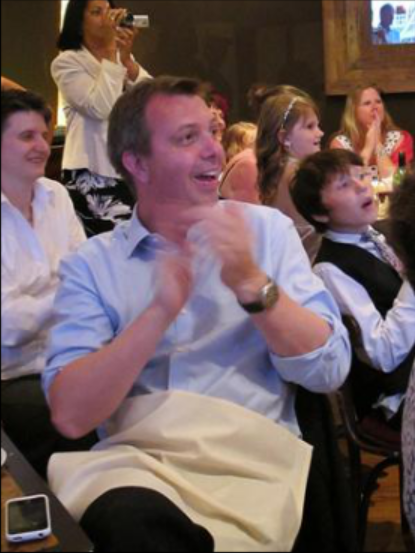
\includegraphics[width=0.24\textwidth]{ensan_salem}\label{fig:ensan_salem}}
 	\hfill
 	\subfloat[بخش بریده شده انسان]{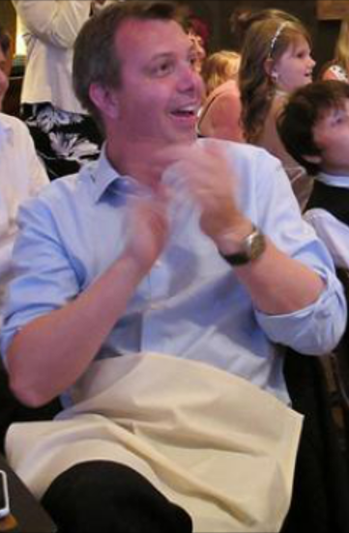
\includegraphics[width=0.22\textwidth]{ensan_boride}\label{fig:ensan_boride}}
 	\hfill
 	\subfloat[نقاط کلیدی بدن انسان]{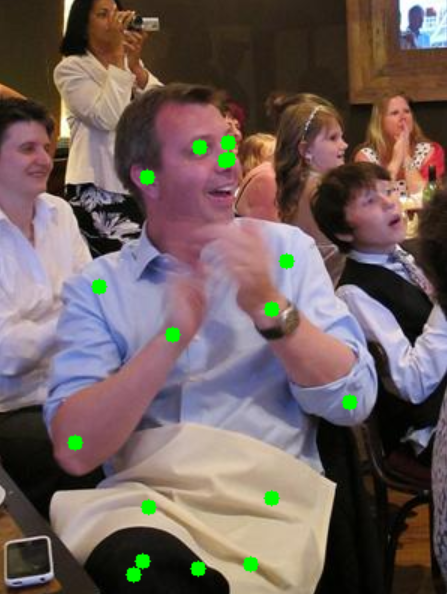
\includegraphics[width=0.24\textwidth]{ensan_nogat}\label{fig:ensan_nogat}}
 	\caption{روند کلی بدست آوردن نقاط کلیدی بدن}
 	\label{fig:koli_ensan_nogte}
 \end{figure}
 به کمک این نقاط کلیدی، %
 \glspl{BoundingBox}
  اجزای بدن ساخته می‌شود. جدول %
 \ref{tab:jadval_nahiye}
 استفاده از نقاط کلیدی مختلف را در راستای ساخت اجزاء بدن نشان می‌دهد.\\
 
  \begin{table}[ht]
 	\centering
 	\onehalfspacing
 	\arrayrulecolor{black}
 	\begin{tabular}{ l | c}
 		\rowcolor{gray}
 		\mrh{نقاط کلیدی}  & \mrh{ناحیه محاسبه شده}     \\
 		\rowcolor{gray!10} مچ دست، آرنج & مچ دست \\
 		\hline شانه، آرنج و مچ دست & آرنج \\
 		\hline
 		\rowcolor{gray!10} مچ پا، زانو & پا \\
 		\hline لگن، زانو و مچ پا & زانو \\
 	\end{tabular}
 	\caption{محاسبه نواحی بدن}
 	\label{tab:jadval_nahiye}
 \end{table}
دربرخی از تصاویر ممکن است بخشی از اجزاء بدن دچار انسداد شده باشد. به جای این بخش‌ها می‌توان فقط صفحه سفید به شبکه ارسال کرد اما در این حالت شبکه دقت پایینی را در هنگام استفاده از آن ثبت می‌کند. بنابراین برای حل این مشکل، ناحیه‌ای که انسان درآن قرار دارد به 9 بخش تقسیم می‌شود و یک بخش از آن به صورت انتخابی از بین این بخش‌ها انتخاب شده و به جای آن قسمت انسداد شده در شبکه حضور پیدا می‌کند.

همچنین مواقعی پیش می‌آید که فقط یکی از نقاط کلیدی مانند "زانو" را دراختیار داریم و فقط با داشتن یک نقاط کلیدی نمی‌توان ناحیه‌ای رسم کرد بدون اینکه فاصله زانو تا مچ پا را درنظر نگیرد، بنابراین دراین حالت‌ها با یک ضریب ثابت و درنظر گرفتن طول %
\gls{BoundingBox}
 انسان در تصویر، اقدام به محاسبه ناحیه مدنظر گرفته شده است.
  \begin{figure}
	\centering
	\subfloat[ ]{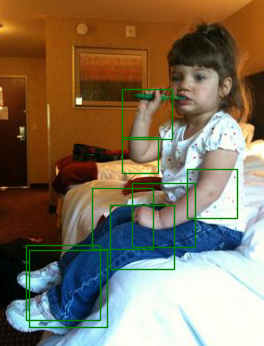
\includegraphics[width=0.22\textwidth]{keypoint_boxes1}\label{fig:keypoint_boxes1}}
	\hfill
	\subfloat[ ]{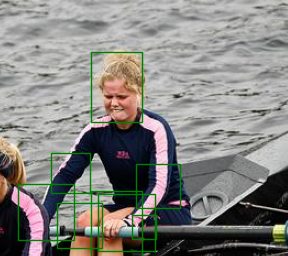
\includegraphics[width=0.28\textwidth]{keypoint_boxes2}\label{fig:keypoint_boxes2}}
	\hfill
	\subfloat[ ]{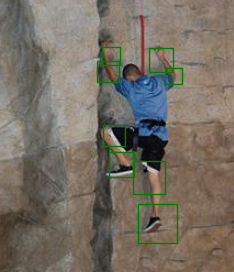
\includegraphics[width=0.22\textwidth]{keypoint_boxes3}\label{fig:keypoint_boxes3}}
	\caption{تصاویر ناحیه احاطه کننده ژست بدست آمده از نقاط کلیدی}
	\label{fig:keypoint_boxes}
\end{figure}

در محاسبه ناحیه‌های، ناحیه "بدن" و "سر" درنظر نگرفته شده است، به این دلیل که ناحیه بدن اطلاعات خاصی را به شبکه اضافه نمی‌کند همچنین ناحیه سر نیز چندان در تشخیص فعالیت تاثیرگذار نیست.

شاید سوال باشد که در تصویر %
\ref{fig:keypoint_boxes2}
 ناحیه "سر" انتخاب شده ولی این ناحیه به جای ناحیه پا که دچار اسنداد شده به صورت جایگزین انتخاب شده است، زیرا همانطور که گفتیم یک ناحیه از انسان به صورت شانسی انتخاب خواهد شد و دراینجا سر انتخاب شده است
 \subsection{تعامل ژست در مکانیزم توجه}
مکانیزم توجه امکان اختصاص وزن‌های مختلف به نقاط مختلف تصویر را فراهم کرده و به شبکه‌های عصبی اجازه می‌دهد تا به نقاط مهم و حیاتی تصویر با دقت بیشتری توجه کنند. طبق این موضوع، شبکه سعی می‌‌کند ارتباط بین انسان و اشیاء که در فعالیت دخیل هستند پیدا کند. دربیشتر روش‌های تشخیص فعالیت انسان، ژست کمترین اهمیت را داشته و اصولاً این ویژگی مهم را درنظر گرفته نشده است. 
 \subsection{بخش اول: مسیر توصیف کننده زاویه بدن }
 در این بخش با استفاده از توصیف کننده زاویه بدن،‌ یک برداری بدست می‌آید که خاصیت کامل ژست انسان را توصیف می‌کند. این بردار درترکیب با خروجی بخش ارتباط‌سنج انسان و اشیاء، جهت امتیاز‌دهی و کلاس بندی استفاده می‌شود.
 
 توصیف کننده زاویه بدن، یک اسکلت از ساختار بدن انسان را تشکیل می‌دهد و اطلاعات جامع از بدن انسان استخراج می‌کند. این کار ویژگی‌های مفهومی %
\gls{High-Level}
  از تصویر را فاش ‌می‌کند و درمواقعی که ممکن است انسداد یا پوشیدگی توسط لباس باعث شود قسمتی از بدن از دسترس خارج شود، کاربرد دارد و عملکرد مدل را بهبود می‌بخشد. 
  
برای ساخت بردار ویژگی از اسکلت، اول از نقاط کلیدی که از شبکه MMPose بدست آمده، استفاده شده است. 13 نقطه کلیدی از بدن انتخاب شده است تا در ساخت بردار حرکتی بدن استفاده شود. با این نقاط یک مجموعه از بردارهای جهت‌دار بدن 
 $\left\{\mathbf{v}_l\right\}_{l=1}^L$
 ساخته شده است،‌ که در اینجا 
 .$\mathbf{v}_l \in \mathbb{R}^2$
 و L به تعداد اعضای بدن اشاره دارند.
 
 \begin{figure}[ht]
 	\centerline{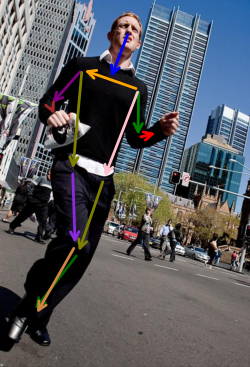
\includegraphics[width=0.28\textwidth]{limb_angle}}
 	\caption{یک نمونه توصیف کننده زاویه بدن}
 	\label{fig:limb_angle}
 \end{figure}

 همانطور که در تصویر %
 \ref{fig:limb_angle}
 مشاهده می‌کنید،‌ 12 بردار شامل 
 \textit{بالا تنه، }
 \textit{شانه، }
\textit{بازو، }
\textit{ساعد، }
\textit{بدن، }
\textit{ران پا و }
\textit{ساق پا}
می‌باشد. جهت این بردارها به کمک دو جفت نقطه کلیدی تعیین شده است.
 طبق فرمول %
 \ref{eq:angle_limb}
 بردار %
 $\mathbf{x}_l^1$
  و بردار %
   $\mathbf{x}_l^2$
 دو تا بردار نشان دهنده یک عضو هستند که با کمک این فرمول بردار جهت‌دار آن بدست آمده است.
\begin{equation}
	\label{eq:angle_limb}
	\mathbf{v}_l=\frac{\left(\mathbf{x}_l^2-\mathbf{x}_l^1\right)}{\left\|\mathbf{x}_l^2-\mathbf{x}_l^1\right\|_2}
\end{equation}

همچنین زاویه بین بردار نشان‌دهنده دو عضو بدن %
   $\mathbf{v}_{l_1}$
   و 
    $\mathbf{v}_{l_2}$
 ، از فرمول %
\ref{eq:angle_bet_limb}
  بدست آمده است.
  \begin{equation}
  	\label{eq:angle_bet_limb}
  	a_{l_1, l_2}=\mathbf{v}_{l_1}^T \cdot \mathbf{v}_{l_2}
  \end{equation}
 در این فرمول ضرب داخلی جفت بردارهای عضو بدن محاسبه شده است، ازاین‌رو از ترکیب جفت تمامی 13 نقطه کلیدی باهم یک بردار به طول 78 تولید شده است (%
  $C_{13}^2=78$
  ). از روی این بردار یک بردار عضو بدن بهینه محاسبه شده است که از ترکیب جفت تمامی 78 تایی بردار با یکدیگر است که درنهایت باعث ساخت یک بردار ویژگی توصیف کننده بدن بهینه به طول 3003 شده است که ویژگی‌های بیشتر و بهینه‌تری از ژست را توصیف می‌کند(
    $C_{78}^2=3003$
  ). این ویژگی بهینه می‌تواند نیاز مدل را به حد کافی برآورده کند. %
  \cite{Recognition_fusing_mutple_cue}
  
  بردار ساخته شده درآخر با خروجی بخش ارتباط‌سنج انسان و اشیاء ترکیب شده و وارد بخش نهایی برای امتیاز‌دهی می‌شود و تعیین می‌گردد که به کدام فعالیت تعلق دارد.
  
   \subsection{بخش دوم: مسیر ارتباط‌سنج انسان و ژست}
   
 ابتدا باید تشخیص داده شود که کدام ویژگی باید با ژست ترکیب شود؟ آیا ترکیب ویژگی‌های اشیاء با ژست نتیجه بهتری می‌دهد یا موقعیت بدنی با ژست؟ در جواب باید گفت که ترکیب ویژگی‌های موقعیت بدنی انسان با ژست انتخاب معقول‌تری است. زیرا ارتباط بین اشیاء و ژست حتی برای انسان نیز چندان واضح نیست. علاوه‌ بر این در ارتباط بین موقعیت بدنی و اشیاء، این ارتباط تا حد زیادی شکل گرفته است و اضافه کردن این ارتباط فقط حجم محاسبات در شبکه را زیاد خواهد کرد و باعث افزایش اطلاعات زائد می‌شود. از این رو دراین پژوهش انتخاب ما ترکیب با موقعیت بدنی است.
 
  ترکیب ویژگی‌های موقعیت بدنی انسان با ژست کمک می‌کند که آن دسته از فعالیت‌هایی که بیشتر با ژست درگیر هستند می‌آید، درآنها اعضای بدن در یک نوع دید محلی درشبکه درنظرگرفته شوند و درنهایت توصیف بهتری از فعالیت درحال انجام به ثمر برسد.
 
 با کمک مکانیزم توجه یکسری ویژگی‌های معنادار و مرتبط بین اجزای ورودی یافت می‌شود. مختصات ژست و ناحیه بدن یا اشیاء به عنوان ورودی‌ در این بخش درنظر گرفته شده است که در داخل یک شبکه ارتباط‌سنج با یکدیگر ترکیب شده و باعث غنی‌تر شدن و بهبود ویژگی‌های مرتبط بین اجزاء مختلف می‌شود. همچنین برخی ویژگی‌های نهفته در تصویر که به سادگی قابل استخراج نیست با کمک این بخش استخراج می‌شود. شکل %
 \ref{fig:majule}
 که از مقاله %
 \cite{Human_object_relation_action}
 الهام گرفته شده است،
 ساختار ماژول ارتباط‌سنج را نشان می‌دهد که ترکیب ویژگی‌های انسان با ژست و انسان با اشیاء را انجام می‌دهد. 
  \begin{figure}[ht]
 	\centerline{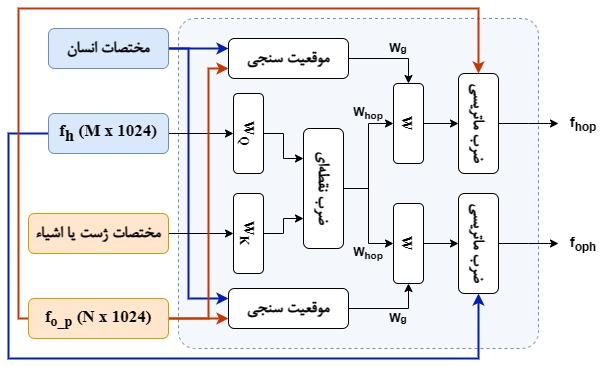
\includegraphics[width=0.7\textwidth]{majule}}
 	\caption{جزییات ساختار ماژول ارتباط‌سنج}
 	\label{fig:majule}
 \end{figure}
 
 به عنوان ورودی در این ماژول ویژگی‌های انسان، ژست و اشیاء درکنار 
 \glspl{BoundingBox}
 آنها داده می‌شود و درخروجی ویژگی ترکیب شده انسان با ژست و انسان با اشیاء دریافت می‌شود. این ماژول ارتباط دوتایی را پیدا می‌کند،‌ از این رو وزن هایی که به هرکدام از روابط (مانند انسان با ژست و انسان با اشیاء) اختصاص داده می‌شود، متفاوت خواهد بود. در ادامه محاسبات انجام شده در داخل این ماژول شرح داده شده است:
 
 طبق فرمول %
 \ref{eq:ebarat_softmax}
  ورودی‌ها متشکل از بردار ویژگی انسان %
  $f_h$
   و بردار ویژگی اشیاء و یا بردار ویژگی ژست %
    $f_{o-p}$ 
    می‌باشد که درهم ضرب نقطه‌ای می‌شوند و خروجی وزن‌دار تولید می‌کنند.
 \begin{equation}
 	\label{eq:ebarat_softmax}
 	w_{hop}=\operatorname{softmax}\left(\frac{W_Q f_h \cdot W_K f_{o-p}}{\sqrt{d_k}}\right)
 \end{equation}
 در اینجا %
 $d_k$
 به عنوان یک %
\gls{ScalingFactor}
درنظر گرفته شده که گرادیان‌های پایدارتری در فاز آموزش داشته باشیم. \\
ارتباط بین انسان با ژست و انسان با اشیاء، تنها به ویژگی‌های آنها مربوط نمی‌شود بلکه به موقعیت مکانی آنها نیز بستگی دارد. بنابراین از موقعیت هندسی مرتبط با آنها نیز استفاده شده است که %
\gls{PositionEmbedding}
 صورت گیرد.
\begin{equation}
	\label{eq:scaling_factor}
	w_g=f c\left(\varepsilon_g\left(b_h, b_{o-p}\right)\right)
\end{equation}
 در اینجا %
 $f c$
 یک لایه %
\gls{FullyConnected}
،‌ %
 $b_h$
 \gls{BoundingBox}
  انسان و %
 $b_{o-p}$
 \gls{BoundingBox}
 اعضاء بدن و اشیاء را نشان می‌دهد که در یک عملیات موقعیت‌سنجی   %
 $\varepsilon_g$
 موقعیت هندسی آن‌ها محاسبه می‌شود. برای اینکه وزن‌هایی که از طریق موقعیت هندسی بدست آمده نسبت به اندازه و %
\gls{Translation}
  مقاوم باشد، ناحیه‌ای که درآن ارتباط دارند از طریق فرمول %
  \ref{eq:postion_embed}
   بدست آمده است:
\begin{equation}
	\label{eq:postion_embed}
	\left(\log \left(\frac{\left|x_h-x_{o-p}\right|}{w_h}\right)\right), \log \left(\frac{\left|y_h-y_{o-p}\right|}{h_h}\right), \log \left(\frac{w_{o-p}}{w_h}\right), \log \left(\frac{h_{o-p}}{h_h}\right)
\end{equation}
با اعمال این تغییرات روی 
 \glspl{BoundingBox}
 اصلی، مقادیر و مختصات جدیدی بدست ‌می‌آید که درنهایت این مقادیر در روند شبکه، مورد استفاده قرار می‌گیرد 
\cite{Relation_network_object}
.
 
 خروجی %
  $w_{hop}$
  که از فرمول %
 \ref{eq:ebarat_softmax}
  و مقدار %
 $w_g$
 که در از فرمول %
 \ref{eq:scaling_factor}
 بدست آمده است و همچنین ویژگی‌هایی که از بخش مختصات اشیاء و ژست بدست آمده است در یک روند ارتباط‌سنجی باهم ترکیب می‌شوند و خروجی بهینه شده بدست می‌آید:
 \begin{equation}
 	f_{h o p}=f c\left(\sum_{i=1}^n\left(\left(w_g w_{h op}\right) \cdot f_{o p}\right)\right)
 \end{equation}
شکل %
   \ref{fig:joziyat_bishtar}
   یک ساختار کلی‌تری از نحوه تشکیل شبکه در داخل بخش ارتباط‌سنج را نشان می‌دهد. 
     \begin{figure}[ht]
   	\centerline{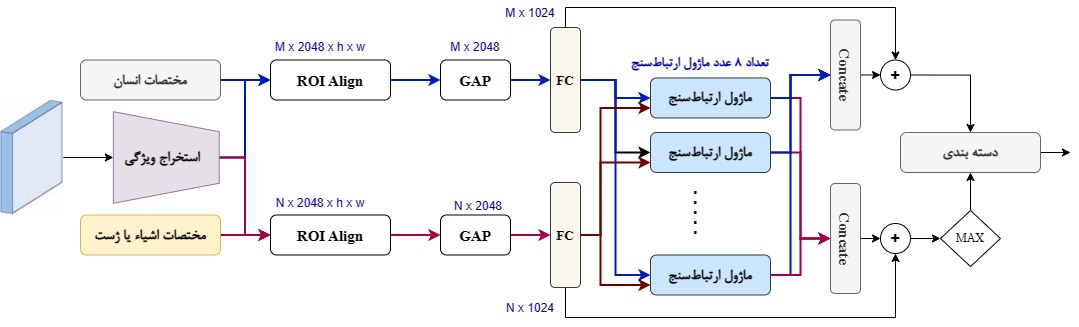
\includegraphics[width=0.95\textwidth]{joziyat_bishtar}}
   	\caption{نگاه کلی‌تر به ساختار بخش ارتباط‌سنج}
   	\label{fig:joziyat_bishtar}
   \end{figure}
ابتدا تصویر وارد شبکه ResNet می‌شود که استخراج ویژگی‌ کلی از تصویر انجام گیرد. سپس از یک بخش %
\lr{RoI Align}
 می‌گذرد که ویژگی‌های ناحیه خاص از تصویر استخراج شود. در مسیر اول ویژگی‌های تصویر با کمک مختصات موقعیت بدنی انسان، خروجی مختص به بخشی از تصویر که انسان درآن حضور دارد را ‌می‌دهد. همینطور در مسیر دوم، خروجی‌ها بادرنظرگرفتن ناحیه اشیاء یا ژست تولید خواهد شد. سپس از یک GAP%
 \LTRfootnote{Global Average Pooling}
 رد می‌شود که ویژگی‌ها یک مقدار فشرده‌تر شود. درنهایت از یک لایه FC%
 \LTRfootnote{Fully Connected}
 می‌گذرد تا بار دیگر ترکیب انجام شود. سپس از چندین ماژول ارتباط‌سنج گذر می‌کند. تعداد ماژول ها 8 عدد درنظر گرفته می‌شود که از معماری %
   \gls{MultHeadAttention}
 استفاده می‌کند (
   $N_r=8$
  ). استفاده از معماری %
     \gls{MultHeadAttention}
  به شبکه این قابلیت را می‌دهد که از فضاها و دید‌های مختلف به داده نگاه کند. همچنین قابلیت موازی سازی را به شبکه اضافه می‌کند.مقدار %
   $d_k*N_r$
   برابر با اندازه بردار ویژگی‌های ورودی (1024) می‌باشد. در نهایت همه‌ خروجی‌های معماری چند شاخه به هم %
\gls{Concatenate}
    می‌شوند. البته در بخش پایین که از ژست یا اشیاء استفاده می‌شود از Max استفاده شده که یک شیء یا یک
عضو بدن در ژست که بیشترین ارتباط را با فعالیت دارد انتخاب شود.
      \subsection{تابع خطا و ترکیب امتیازات}
   بعد از اینکه ورودی از ماژول انسان - ژست و انسان - اشیاء عبور می‌کند که ویژگی‌های مرتبط با یکدیگر استخراج شود و درنهایت خروجی‌های معماری چند شاخه به هم متصل می‌شوند که یک بردار ویژگی واحد را تشکیل دهند. این بردار ویژگی از یک بخش فولی کانکتد می‌گذرد تا وارد بخش امتیازدهی شوند. 
   البته بخش دوم و سوم که مربوط به ویژگی‌های ژست و اشیاء می‌باشد، از یک %
   $max$
   عبور می‌کنند که بیشتر امتیاز بدست آمده درنظر گرفته شود. فرمول نهایی به شکل زیر خواهد بود:
   \begin{equation}
   	\operatorname{Score}(a ; h)=S_h^a+\max \left\{S_{o(1)}^a, \ldots, S_{o(n)}^a\right\}+\max \left\{S_{o(1)}^a, \ldots, S_{o(m)}^a\right\}
   \end{equation}
   
   در نهایت از یک %
   $softmax$
   عبور می‌گذرد که امتیازات ترکیب شده با جمع احتمالات برابر با یک فعالیت مورد نظر را تشخیص دهد. در روند آموزش فقط برچسب نام فعالیت مورد نظر در یک فرآیند خودناظر نیاز است که فعالیت درحال انجام را تشخیص دهد. برای تابع خطا هم از %
   $Cross$ $Entropy$ $Loss$
    استفاده شده است که در ادامه فرمول %
   \ref{eq:loss_function}
   این رابطه را نشان می‌دهد.
   \begin{equation}
   	\label{eq:loss_function}
   	L=-\log \left(\frac{\exp \left(\operatorname{Score}\left(a^{g t} ; h\right)\right)}{\sum_a \exp (\operatorname{Score}(a ; h))}\right)
   \end{equation}
   در اینجا %
    $\operatorname{Score}(a ; h)$
   امتیازات جمع‌آوری شده از فعالیت %
   $a$
   و %
   $g^t$
    در عبارت %
   $\operatorname{Score}\left(a^{g t} ; h\right)$
  نشان دهنده برچسب یا کلاسی است که فعالیت به آن تعلق دارد.